% Header: Theoretical Physics 2 homework solution
%%%%%%%%%%%%%%%%%%%%%%%%%%%%%%%%%%%%%%%%%%%%%%%%%%%%%%%%%%%%%%%%%%%

\documentclass[11pt,a4paper]{scrartcl}

% Layout
\usepackage[margin=2.5cm]{geometry}
\usepackage[onehalfspacing]{setspace}

% General packages
\usepackage{graphicx}
\usepackage{enumitem}
\usepackage{tcolorbox}
\tcbuselibrary{breakable}
\usepackage[breaklinks=true,colorlinks=true,linkcolor=blue,urlcolor=blue,citecolor=blue]{hyperref}
\usepackage{amsmath,amsthm,amssymb,mathtools}
\usepackage{braket}
\usepackage{icomma}
\usepackage[T1]{fontenc}
\usepackage[utf8]{inputenc}
\usepackage[english]{babel}
\usepackage{tikz}

% Units / tables / floats / references
\usepackage[locale = UK,space-before-unit=true,per-mode = symbol]{siunitx}
\usepackage{booktabs,multirow}
\usepackage{placeins}
\usepackage[natbib,abbreviate=true,doi=false,style=numeric-comp,giveninits=true,sorting=none]{biblatex}
\usepackage{csquotes}

% Graphics paths
\graphicspath{{Bilder/} {images/} {figures/} {chapters/}}

% Optional math shortcuts
\newcommand{\R}{\mathbb{R}}
\newcommand{\N}{\mathbb{N}}
\newcommand{\Q}{\mathbb{Q}}
\newcommand{\abs}[1]{\left| #1 \right|}
\newcommand{\norm}[1]{\left\lVert #1 \right\rVert}
\newcommand{\ol}[1]{\overline{#1}}
\newcommand{\ii}{\mathrm{i}}
\newcommand{\e}{\mathrm{e}}
\newcommand{\op}[1]{\hat{#1}}

% Optional units
\DeclareSIUnit{\dBm}{dBm}

% Box styles
\newtcolorbox{calculationbox}[1][]{
    title=Calculation,
    breakable,
    #1
}

\newtcolorbox{solutionbox}[1][]{
    title=Solution,
    breakable,
    #1
}

\newtcolorbox{answerbox}[1][]{
    title=Answer,
    breakable,
    #1
}

\newtcolorbox{notebox}[1][]{
    title=Notes,
    breakable,
    #1
}

\newtcolorbox{sidecalcbox}[1][]{
    title=Side Calculation,
    breakable,
    #1
}

%%%%%%%%%%%%%%%%%%%%%%%%%%%%%%%%%%%%%%%%%%%%%%%%%%%%%%%%%%%%%%%%%%%
\begin{document}

    \title{Theoretical Physics 2 -- Sheet 08}
    \author{Tobias Laser}
    \date{\today}
    \maketitle
    \vfill
    \thispagestyle{empty}
    \newpage

    \pagenumbering{arabic}

    % ================================================================
    \paragraph{19. Time evolution and measurements of a spin with $s=\frac12$}

    We consider a spin-$\frac12$ particle with initial state
    \[
        \ket{\psi(0)} = \ket{\downarrow}.
    \]
    The Hamiltonian is
    \[
        \op{H} = \frac{\hbar\omega}{2}\sigma_x.
    \]

    \begin{enumerate}[label=(\alph*)]
        \item At time $t_1=\frac{\pi}{2\omega}$ the operator $\sigma_z$ is measured. In which state is the particle at this time? Which measurement results are possible, and with which probabilities do they occur?

        \begin{calculationbox}
            The time evolution operator is obtained from the Schrödinger equation by
            \[
                \op{U}(t) = \exp\left(-\frac{\ii}{\hbar}\op{H}t\right)
                = \exp\left(-\ii\frac{\omega t}{2}\sigma_x\right).
            \]
            Since $\sigma_x^2=\mathbb{1}$, the exponential splits into even and odd powers.

            \begin{calculationbox}
                \begin{align*}
                    \op{U}(t)
                    &= \sum_{n=0}^{\infty}\frac{1}{n!}\left(-\ii\frac{\omega t}{2}\sigma_x\right)^n \\
                    &= \mathbb{1}\sum_{k=0}^{\infty}\frac{(-1)^k}{(2k)!}\left(\frac{\omega t}{2}\right)^{2k}
                    -\ii\sigma_x\sum_{k=0}^{\infty}\frac{(-1)^k}{(2k+1)!}\left(\frac{\omega t}{2}\right)^{2k+1} \\
                    &= \mathbb{1}\cos\left(\frac{\omega t}{2}\right)
                    -\ii\sigma_x\sin\left(\frac{\omega t}{2}\right).
                \end{align*}
            \end{calculationbox}

            At $t_1=\frac{\pi}{2\omega}$ this gives $\frac{\omega t_1}{2}=\frac{\pi}{4}$, hence
            \begin{calculationbox}
                \begin{align*}
                    \ket{\psi(t_1)}
                    &= \left[\mathbb{1}\cos\left(\frac{\pi}{4}\right)-\ii\sigma_x\sin\left(\frac{\pi}{4}\right)\right]\ket{\downarrow} \\
                    &= \frac{1}{\sqrt{2}}\left(\ket{\downarrow}-\ii\ket{\uparrow}\right).
                \end{align*}
            \end{calculationbox}

            The eigenstates of $\sigma_z$ are
            \[
                \sigma_z\ket{\uparrow}=+\ket{\uparrow},
                \qquad
                \sigma_z\ket{\downarrow}=-\ket{\downarrow}.
            \]
            Therefore the two possible measurement results are $+1$ and $-1$.

            \begin{calculationbox}
                \begin{align*}
                    P(+1) &= \abs{\braket{\uparrow|\psi(t_1)}}^2
                    = \abs{-\frac{\ii}{\sqrt{2}}}^2
                    = \frac12, \\
                    P(-1) &= \abs{\braket{\downarrow|\psi(t_1)}}^2
                    = \abs{\frac{1}{\sqrt{2}}}^2
                    = \frac12.
                \end{align*}
            \end{calculationbox}
        \end{calculationbox}

        \begin{answerbox}
            Immediately before the measurement,
            \[
                \boxed{\ket{\psi(t_1)}=\frac{1}{\sqrt{2}}\left(\ket{\downarrow}-\ii\ket{\uparrow}\right)}.
            \]
            A measurement of $\sigma_z$ gives
            \[
                \boxed{+1 \text{ with probability } \frac12, \qquad -1 \text{ with probability } \frac12.}
            \]
            After the measurement the state collapses to $\ket{\uparrow}$ if the result was $+1$, and to $\ket{\downarrow}$ if the result was $-1$.
        \end{answerbox}

        \item Directly after the measurement the system evolves for a time interval $\Delta t=\frac{\pi}{2\omega}$. At time $t_2=t_1+\Delta t=\frac{\pi}{\omega}$, $\sigma_z$ is measured again. Depending on the result from part (a), in which state is the particle at $t_2$, and with which probabilities do the possible results occur?

        \begin{calculationbox}
            After the first measurement, there are two possible collapsed states. For both branches the further time evolution is given by
            \[
                \op{U}(\Delta t)
                = \mathbb{1}\cos\left(\frac{\omega\Delta t}{2}\right)
                -\ii\sigma_x\sin\left(\frac{\omega\Delta t}{2}\right)
                = \frac{1}{\sqrt{2}}(\mathbb{1}-\ii\sigma_x),
            \]
            because $\Delta t=\frac{\pi}{2\omega}$.

            \begin{calculationbox}
                If the first result was $+1$, then directly after the first measurement
                \[
                    \ket{\psi'}=\ket{\uparrow}.
                \]
                Thus
                \begin{align*}
                    \ket{\psi(t_2)}
                    &= \op{U}(\Delta t)\ket{\uparrow} \\
                    &= \frac{1}{\sqrt{2}}(\mathbb{1}-\ii\sigma_x)\ket{\uparrow} \\
                    &= \frac{1}{\sqrt{2}}\left(\ket{\uparrow}-\ii\ket{\downarrow}\right).
                \end{align*}
                Therefore
                \[
                    P(+1\mid +1 \text{ at } t_1)=\frac12,
                    \qquad
                    P(-1\mid +1 \text{ at } t_1)=\frac12.
                \]
            \end{calculationbox}

            \begin{calculationbox}
                If the first result was $-1$, then directly after the first measurement
                \[
                    \ket{\psi'}=\ket{\downarrow}.
                \]
                Thus
                \begin{align*}
                    \ket{\psi(t_2)}
                    &= \op{U}(\Delta t)\ket{\downarrow} \\
                    &= \frac{1}{\sqrt{2}}(\mathbb{1}-\ii\sigma_x)\ket{\downarrow} \\
                    &= \frac{1}{\sqrt{2}}\left(\ket{\downarrow}-\ii\ket{\uparrow}\right).
                \end{align*}
                Therefore
                \[
                    P(+1\mid -1 \text{ at } t_1)=\frac12,
                    \qquad
                    P(-1\mid -1 \text{ at } t_1)=\frac12.
                \]
            \end{calculationbox}
        \end{calculationbox}

        \begin{answerbox}
            In both branches the second measurement has equal probabilities:
            \[
                \boxed{P(+1)=\frac12, \qquad P(-1)=\frac12}
            \]
            conditional on the respective state after the first measurement. The difference between the two branches is the relative phase and which basis vector is written first.
        \end{answerbox}

        \item In contrast to the previous parts, the particle now evolves without interruption until $t_2$. In which state is the particle at this time? Which probabilities result from a measurement of $\sigma_z$ at $t_2$? Explain the difference to part (b).

        \begin{calculationbox}
            Without an intermediate measurement, the state is evolved directly from $t=0$ to $t_2=\frac{\pi}{\omega}$.
            Then
            \[
                \frac{\omega t_2}{2}=\frac{\pi}{2}.
            \]
            Hence
            \begin{calculationbox}
                \begin{align*}
                    \ket{\psi(t_2)}
                    &= \left[\mathbb{1}\cos\left(\frac{\pi}{2}\right)-\ii\sigma_x\sin\left(\frac{\pi}{2}\right)\right]\ket{\downarrow} \\
                    &= -\ii\sigma_x\ket{\downarrow} \\
                    &= -\ii\ket{\uparrow}.
                \end{align*}
            \end{calculationbox}
            The global phase $-\ii$ has no physical effect. Therefore this state is physically the same as $\ket{\uparrow}$.
        \end{calculationbox}

        \begin{answerbox}
            At $t_2$ the state is
            \[
                \boxed{\ket{\psi(t_2)}=-\ii\ket{\uparrow}.}
            \]
            Therefore a measurement of $\sigma_z$ gives
            \[
                \boxed{P(+1)=1, \qquad P(-1)=0.}
            \]
            The difference to part (b) is caused by the intermediate measurement. In part (b), the first measurement destroys the coherent superposition and projects the state onto one of the $\sigma_z$ eigenstates. Without this projection, the amplitudes continue to interfere coherently, and the final state becomes $\ket{\uparrow}$ up to a global phase.
        \end{answerbox}
    \end{enumerate}

    % ================================================================
    \paragraph{20. System with angular momentum $l=1$}

    We consider a system with angular momentum $l=1$. The basis vectors
    \[
        \ket{+1},\quad \ket{0},\quad \ket{-1}
    \]
    are eigenvectors of $\op{L}_z$ with eigenvalues $\hbar,0,-\hbar$. The ladder operators satisfy
    \[
        \op{L}_{\pm}\ket{m}=\hbar\sqrt{2}\ket{m\pm 1},
        \qquad
        \op{L}_{+}\ket{1}=\op{L}_{-}\ket{-1}=0.
    \]
    The Hamiltonian is
    \[
        \op{H}=\frac{\omega_0}{\hbar}\left(\op{L}_u^2-\op{L}_v^2\right),
    \]
    where $\op{L}_u$ and $\op{L}_v$ are the components along the diagonals of the $xz$-plane.

    \begin{enumerate}[label=(\alph*)]
        \item Give the matrix representation of $\op{H}$ in the basis $\{\ket{+1},\ket{0},\ket{-1}\}$. What are the stationary states and their energy eigenvalues? Write them as $\ket{E_1},\ket{E_2},\ket{E_3}$ with $E_1\geq E_2\geq E_3$.

        \begin{calculationbox}
            Since $u$ and $v$ are the diagonals of the $xz$-plane, we use
            \[
                \op{L}_u=\frac{1}{\sqrt{2}}(\op{L}_x+\op{L}_z),
                \qquad
                \op{L}_v=\frac{1}{\sqrt{2}}(\op{L}_z-\op{L}_x).
            \]
            Because operators do not necessarily commute, we expand the squares carefully.

            \begin{calculationbox}
                \begin{align*}
                    \op{L}_u^2-\op{L}_v^2
                    &= \frac12(\op{L}_x+\op{L}_z)^2
                    -\frac12(\op{L}_z-\op{L}_x)^2 \\
                    &= \frac12\left(\op{L}_x^2+\op{L}_x\op{L}_z+\op{L}_z\op{L}_x+\op{L}_z^2\right) \\
                    &\quad -\frac12\left(\op{L}_z^2-\op{L}_z\op{L}_x-\op{L}_x\op{L}_z+\op{L}_x^2\right) \\
                    &= \op{L}_x\op{L}_z+\op{L}_z\op{L}_x.
                \end{align*}
            \end{calculationbox}

            In the ordered basis $(\ket{+1},\ket{0},\ket{-1})$, the matrices are
            \begin{calculationbox}
                \[
                    \op{L}_z
                    =\hbar
                    \begin{pmatrix}
                        1&0&0\\
                        0&0&0\\
                        0&0&-1
                    \end{pmatrix},
                    \qquad
                    \op{L}_x
                    =\frac12(\op{L}_++\op{L}_-)
                    =\frac{\hbar}{\sqrt{2}}
                    \begin{pmatrix}
                        0&1&0\\
                        1&0&1\\
                        0&1&0
                    \end{pmatrix}.
                \]
            \end{calculationbox}

            Therefore
            \begin{calculationbox}
                \begin{align*}
                    \op{H}
                    &=\frac{\omega_0}{\hbar}(\op{L}_x\op{L}_z+\op{L}_z\op{L}_x) \\
                    &=\frac{\hbar\omega_0}{\sqrt{2}}
                    \left[
                    \begin{pmatrix}
                        0&0&0\\
                        1&0&-1\\
                        0&0&0
                    \end{pmatrix}
                    +
                    \begin{pmatrix}
                        0&1&0\\
                        0&0&0\\
                        0&-1&0
                    \end{pmatrix}
                    \right] \\
                    &=\frac{\hbar\omega_0}{\sqrt{2}}
                    \begin{pmatrix}
                        0&1&0\\
                        1&0&-1\\
                        0&-1&0
                    \end{pmatrix}.
                \end{align*}
            \end{calculationbox}

            To diagonalise, write
            \[
                \op{H}=\hbar\omega_0 A,
                \qquad
                A=\frac{1}{\sqrt{2}}
                    \begin{pmatrix}
                        0&1&0\\
                        1&0&-1\\
                        0&-1&0
                    \end{pmatrix}.
            \]
            The characteristic polynomial of $A$ is
            \begin{calculationbox}
                \[
                    \det(A-\lambda\mathbb{1})
                    = -\lambda(\lambda^2-1).
                \]
                Thus
                \[
                    \lambda_1=1,
                    \qquad
                    \lambda_2=0,
                    \qquad
                    \lambda_3=-1.
                \]
            \end{calculationbox}

            The normalized eigenvectors are
            \begin{calculationbox}
                \begin{align*}
                    \ket{E_1}
                    &=\frac12\ket{+1}+\frac{1}{\sqrt{2}}\ket{0}-\frac12\ket{-1},
                    &E_1&=\hbar\omega_0,\\
                    \ket{E_2}
                    &=\frac{1}{\sqrt{2}}\ket{+1}+\frac{1}{\sqrt{2}}\ket{-1},
                    &E_2&=0,\\
                    \ket{E_3}
                    &=\frac12\ket{+1}-\frac{1}{\sqrt{2}}\ket{0}-\frac12\ket{-1},
                    &E_3&=-\hbar\omega_0.
                \end{align*}
            \end{calculationbox}
        \end{calculationbox}

        \begin{answerbox}
            \[
                \boxed{
                \op{H}=\frac{\hbar\omega_0}{\sqrt{2}}
                    \begin{pmatrix}
                        0&1&0\\
                        1&0&-1\\
                        0&-1&0
                    \end{pmatrix}}
            \]
            with stationary states and energies
            \[
                \boxed{
                \begin{aligned}
                    \ket{E_1}&=\frac12\ket{+1}+\frac{1}{\sqrt{2}}\ket{0}-\frac12\ket{-1}, & E_1&=\hbar\omega_0,\\
                    \ket{E_2}&=\frac{1}{\sqrt{2}}(\ket{+1}+\ket{-1}), & E_2&=0,\\
                    \ket{E_3}&=\frac12\ket{+1}-\frac{1}{\sqrt{2}}\ket{0}-\frac12\ket{-1}, & E_3&=-\hbar\omega_0.
                \end{aligned}}
            \]
        \end{answerbox}

        \item At time $t=0$ let the system be in the state
        \[
            \ket{\psi(0)}=\frac{1}{\sqrt{2}}\left(\ket{+1}-\ket{-1}\right).
        \]
        What is the state vector $\ket{\psi(t)}$? At time $t$, $\op{L}_z$ is measured. What are the probabilities for the different possible results?

        \begin{calculationbox}
            First we express the initial state in the energy eigenbasis. Using the eigenvectors from part (a),
            \begin{calculationbox}
                \[
                    \ket{\psi(0)}
                    =\frac{1}{\sqrt{2}}\left(\ket{E_1}+\ket{E_3}\right).
                \]
            \end{calculationbox}
            The time evolution in the energy eigenbasis is diagonal:
            \begin{calculationbox}
                \begin{align*}
                    \ket{\psi(t)}
                    &=\frac{1}{\sqrt{2}}
                    \left(\e^{-\ii E_1t/\hbar}\ket{E_1}
                    +\e^{-\ii E_3t/\hbar}\ket{E_3}\right) \\
                    &=\frac{1}{\sqrt{2}}
                    \left(\e^{-\ii\omega_0t}\ket{E_1}
                    +\e^{\ii\omega_0t}\ket{E_3}\right).
                \end{align*}
            \end{calculationbox}
            Let $\theta=\omega_0t$. Transforming back to the $\op{L}_z$ basis gives
            \begin{calculationbox}
                \begin{align*}
                    \ket{\psi(t)}
                    &=\frac{\cos\theta}{\sqrt{2}}\ket{+1}
                    -\ii\sin\theta\ket{0}
                    -\frac{\cos\theta}{\sqrt{2}}\ket{-1} \\
                    &=\frac{\cos(\omega_0t)}{\sqrt{2}}\left(\ket{+1}-\ket{-1}\right)
                    -\ii\sin(\omega_0t)\ket{0}.
                \end{align*}
            \end{calculationbox}
            A measurement of $\op{L}_z$ can give the eigenvalues $\hbar,0,-\hbar$. The probabilities are the squared moduli of the corresponding coefficients.
            \begin{calculationbox}
                \begin{align*}
                    P(L_z=\hbar) &= \frac12\cos^2(\omega_0t),\\
                    P(L_z=0) &= \sin^2(\omega_0t),\\
                    P(L_z=-\hbar) &= \frac12\cos^2(\omega_0t).
                \end{align*}
            \end{calculationbox}
        \end{calculationbox}

        \begin{answerbox}
            \[
                \boxed{\ket{\psi(t)}=\frac{\cos(\omega_0t)}{\sqrt{2}}\left(\ket{+1}-\ket{-1}\right)-\ii\sin(\omega_0t)\ket{0}}
            \]
            and
            \[
                \boxed{
                P(\hbar)=\frac12\cos^2(\omega_0t),\qquad
                P(0)=\sin^2(\omega_0t),\qquad
                P(-\hbar)=\frac12\cos^2(\omega_0t).}
            \]
        \end{answerbox}

        \item Calculate the expectation values $\langle\op{L}_x(t)\rangle$, $\langle\op{L}_y(t)\rangle$ and $\langle\op{L}_z(t)\rangle$. Which motion does the vector $\langle\op{L}(t)\rangle$ perform? Sketch the trajectory of $\langle\op{L}(t)\rangle$.

        \begin{calculationbox}
            We use the state from part (b), written as a column vector in the ordered basis $(\ket{+1},\ket{0},\ket{-1})$:
            \[
                \ket{\psi(t)}=
                \begin{pmatrix}
                    \frac{\cos\theta}{\sqrt{2}}\\
                    -\ii\sin\theta\\
                    -\frac{\cos\theta}{\sqrt{2}}
                \end{pmatrix},
                \qquad
                \theta=\omega_0t.
            \]
            The angular momentum matrices are
            \begin{calculationbox}
                \[
                    \op{L}_x=\frac{\hbar}{\sqrt{2}}
                    \begin{pmatrix}
                        0&1&0\\
                        1&0&1\\
                        0&1&0
                    \end{pmatrix},
                    \qquad
                    \op{L}_y=\frac{\hbar}{\sqrt{2}}
                    \begin{pmatrix}
                        0&-\ii&0\\
                        \ii&0&-\ii\\
                        0&\ii&0
                    \end{pmatrix},
                    \qquad
                    \op{L}_z=\hbar
                    \begin{pmatrix}
                        1&0&0\\
                        0&0&0\\
                        0&0&-1
                    \end{pmatrix}.
                \]
            \end{calculationbox}

            For $\op{L}_z$, the probabilities of $m=+1$ and $m=-1$ are equal, hence the contributions cancel:
            \begin{calculationbox}
                \[
                    \langle\op{L}_z(t)\rangle
                    =\hbar\frac{\cos^2\theta}{2}-\hbar\frac{\cos^2\theta}{2}=0.
                \]
            \end{calculationbox}

            For $\op{L}_x$, the contributions from the $\ket{+1}\leftrightarrow\ket{0}$ and $\ket{0}\leftrightarrow\ket{-1}$ terms cancel because the coefficients of $\ket{+1}$ and $\ket{-1}$ have opposite signs:
            \begin{calculationbox}
                \[
                    \langle\op{L}_x(t)\rangle=0.
                \]
            \end{calculationbox}

            For $\op{L}_y$, we compute explicitly:
            \begin{calculationbox}
                \begin{align*}
                    \op{L}_y\ket{\psi(t)}
                    &=\frac{\hbar}{\sqrt{2}}
                    \begin{pmatrix}
                        -\ii(-\ii\sin\theta)\\
                        \ii\frac{\cos\theta}{\sqrt{2}}-\ii\left(-\frac{\cos\theta}{\sqrt{2}}\right)\\
                        \ii(-\ii\sin\theta)
                    \end{pmatrix} \\
                    &=
                    \begin{pmatrix}
                        -\frac{\hbar\sin\theta}{\sqrt{2}}\\
                        \ii\hbar\cos\theta\\
                        \frac{\hbar\sin\theta}{\sqrt{2}}
                    \end{pmatrix}.
                \end{align*}
                Hence
                \begin{align*}
                    \langle\op{L}_y(t)\rangle
                    &=
                    \begin{pmatrix}
                        \frac{\cos\theta}{\sqrt{2}} & \ii\sin\theta & -\frac{\cos\theta}{\sqrt{2}}
                    \end{pmatrix}
                    \begin{pmatrix}
                        -\frac{\hbar\sin\theta}{\sqrt{2}}\\
                        \ii\hbar\cos\theta\\
                        \frac{\hbar\sin\theta}{\sqrt{2}}
                    \end{pmatrix} \\
                    &= -\frac{\hbar}{2}\sin\theta\cos\theta
                    -\hbar\sin\theta\cos\theta
                    -\frac{\hbar}{2}\sin\theta\cos\theta \\
                    &= -2\hbar\sin\theta\cos\theta \\
                    &= -\hbar\sin(2\theta).
                \end{align*}
            \end{calculationbox}
        \end{calculationbox}

        \begin{answerbox}
            \[
                \boxed{\langle\op{L}_x(t)\rangle=0,
                \qquad
                \langle\op{L}_y(t)\rangle=-\hbar\sin(2\omega_0t),
                \qquad
                \langle\op{L}_z(t)\rangle=0.}
            \]
            Therefore
            \[
                \boxed{\langle\op{\mathbf{L}}(t)\rangle=(0,-\hbar\sin(2\omega_0t),0).}
            \]
            The expectation value vector oscillates on the $y$-axis between $-\hbar\mathbf{e}_y$ and $+\hbar\mathbf{e}_y$ with angular frequency $2\omega_0$.

            \begin{center}
            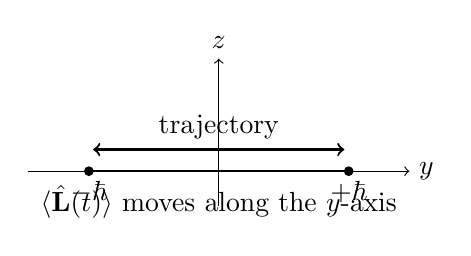
\begin{tikzpicture}[scale=1.1]
                \draw[->] (-2.2,0) -- (2.2,0) node[right] {$y$};
                \draw[->] (0,-0.4) -- (0,1.3) node[above] {$z$};
                \draw[thick] (-1.5,0) -- (1.5,0);
                \fill (-1.5,0) circle (1.6pt) node[below] {$-\hbar$};
                \fill (1.5,0) circle (1.6pt) node[below] {$+\hbar$};
                \draw[<->,thick] (-1.45,0.25) -- (1.45,0.25) node[midway,above] {trajectory};
                \node at (0,-0.35) {$\langle\op{\mathbf{L}}(t)\rangle$ moves along the $y$-axis};
            \end{tikzpicture}
            \end{center}
        \end{answerbox}

        \item At time $t$, a measurement of $\op{L}_z^2$ is performed.
        \begin{enumerate}[label=(\roman*)]
            \item Are there times at which only one single result is possible?
            \item Assume that the measurement gives the result $\hbar^2$. In which state is the system immediately after the measurement? Describe the subsequent evolution without calculation.
        \end{enumerate}

        \begin{calculationbox}
            The operator $\op{L}_z^2$ has eigenvalues
            \[
                \op{L}_z^2\ket{+1}=\hbar^2\ket{+1},
                \qquad
                \op{L}_z^2\ket{0}=0,
                \qquad
                \op{L}_z^2\ket{-1}=\hbar^2\ket{-1}.
            \]
            Thus the result $\hbar^2$ corresponds to the two-dimensional subspace spanned by $\ket{+1}$ and $\ket{-1}$, while the result $0$ corresponds to the one-dimensional subspace spanned by $\ket{0}$.

            From part (b),
            \[
                \ket{\psi(t)}
                =\frac{\cos(\omega_0t)}{\sqrt{2}}(\ket{+1}-\ket{-1})
                -\ii\sin(\omega_0t)\ket{0}.
            \]
            Hence
            \begin{calculationbox}
                \begin{align*}
                    P(L_z^2=\hbar^2) &= \cos^2(\omega_0t),\\
                    P(L_z^2=0) &= \sin^2(\omega_0t).
                \end{align*}
            \end{calculationbox}

            Therefore only one result is possible when one of these probabilities is equal to $1$.
            \begin{calculationbox}
                \begin{align*}
                    P(L_z^2=\hbar^2)=1
                    &\Longleftrightarrow \cos^2(\omega_0t)=1
                    \Longleftrightarrow \omega_0t=n\pi, \\
                    &\Longleftrightarrow t=\frac{n\pi}{\omega_0},\quad n\in\mathbb{Z},\\[0.4em]
                    P(L_z^2=0)=1
                    &\Longleftrightarrow \sin^2(\omega_0t)=1
                    \Longleftrightarrow \omega_0t=\frac{\pi}{2}+n\pi, \\
                    &\Longleftrightarrow t=\frac{\pi}{2\omega_0}+\frac{n\pi}{\omega_0},\quad n\in\mathbb{Z}.
                \end{align*}
            \end{calculationbox}

            If the measurement gives $\hbar^2$, we project onto the subspace spanned by $\ket{+1}$ and $\ket{-1}$ and then normalize.
            \begin{calculationbox}
                \begin{align*}
                    \op{P}_{\hbar^2}\ket{\psi(t)}
                    &=\frac{\cos(\omega_0t)}{\sqrt{2}}(\ket{+1}-\ket{-1}),\\
                    \ket{\psi_{\text{after}}}
                    &=\frac{\op{P}_{\hbar^2}\ket{\psi(t)}}{
orm{\op{P}_{\hbar^2}\ket{\psi(t)}}}
                    =\frac{1}{\sqrt{2}}(\ket{+1}-\ket{-1}),
                \end{align*}
            \end{calculationbox}
            up to an irrelevant overall phase. This is the same form as the initial state in part (b).
        \end{calculationbox}

        \begin{answerbox}
            \begin{enumerate}[label=(\roman*)]
                \item Yes. For
                \[
                    \boxed{t=\frac{n\pi}{\omega_0}}
                \]
                only the result $\hbar^2$ is possible. For
                \[
                    \boxed{t=\frac{\pi}{2\omega_0}+\frac{n\pi}{\omega_0}}
                \]
                only the result $0$ is possible.

                \item If the result is $\hbar^2$, the state immediately after the measurement is
                \[
                    \boxed{\ket{\psi_{\text{after}}}=\frac{1}{\sqrt{2}}(\ket{+1}-\ket{-1})}
                \]
                up to a global phase. Since this is the same state as the initial state in part (b), the subsequent time evolution repeats the same oscillation: probability is periodically transferred between the $\hbar^2$ subspace and the $0$ eigenstate $\ket{0}$.
            \end{enumerate}
        \end{answerbox}
    \end{enumerate}

\end{document}
